\documentclass[xcolor={usenames,svgnames,x11names,dvipsnames,table}]{beamer}

\usetheme{SBUclass}

\usepackage{mypackages}
\usepackage{mycommands}

\title{\texorpdfstring{Language \& Technology}{Language and Technology}}
\subtitle{Lecture 8: A Glimpse at More Adequate Models}
\author{Thomas Graf}
\institute{Stony Brook University\\\texttt{lin120@thomasgraf.net}}
\date{}


\begin{document}
\unnumbered{
\begin{frame}
	\titlepage
\end{frame}
}

\begin{frame}{Current Model}
    \highlight{$n$-gram models} rule the field.
    %
    \begin{description}
        \item[word n-gram] sequence of $n$ words
        \item[character n-gram] sequence of $n$ characters
    \end{description}
    %
    \begin{example}
        \begin{tabular}{rl}
            \textbf{Sentence} & Mary really really likes Marty\\[12pt]
            %
            \textbf{Word trigrams} & Mary really really\\
            \textbf{(types)}       & really really likes\\
                                   & really likes Marty\\[12pt]
            %
            \textbf{Char trigrams} & Mar, ary, ry\_, y\_r,\\
            \textbf{(types)}       & \_re, rea, eal, all, lly, ly\_, y\_l,\\
                                   & \_li, lik, ike, kes, es\_, s\_M\\
                                   & \_Ma, art, rty
        \end{tabular}
    \end{example}
\end{frame}

\begin{frame}{Applications of $n$-Grams}
    \begin{itemize}
        \item word completion \& prediction
        \item context in spell checking\\
              \subpoint{good ``there are'' VS bad ``their are''}
        \item possible word detection in spell checking\\
              \subpoint{does the word contain only possible bigrams of English?}
        \item word choice in OCR\\
              \subpoint{pick word that maximizes sentence probability}
    \end{itemize}
\end{frame}

\begin{frame}{Modus operandi}
    \begin{enumerate}
        \item Collect large corpus
        \item Extract all bi-\slash tri\slash n-gram types and their counts
        \item Convert counts to frequency
        \item Compute probabilities of relevant alternatives\\
              \subpoint{e.g.\ possible word completions}
        \item Pick choice with highest probability
    \end{enumerate}
\end{frame}

\begin{frame}{Example of Probability Maximization}
    \begin{tabular}{rl}
        \textbf{Alternatives} & \textbf{A)} John wants to be happy.\\
                              & \textbf{B)} John wants to he happy.\\[12pt]

        \textbf{Bigram probabilities} & John wants: 2\%\\
                                      & wants to: 5\%\\
                                      & to be: 10\%\\
                                      & to he: 1\%\\
                                      & be happy: 5\%\\
                                      & he happy: 1\%\\
    \end{tabular}

    \pause
    \begin{align*}
        P(\text{A}) &= P(\text{John wants}) \times
                       P(\text{wants to}) \times
                       P(\text{to be}) \times
                       P(\text{be happy})\\ 
                    &= 2\% \times 5\% \times 10\% \times 5\%\\
                    &= 0.005\%
    \end{align*}
    %
    \begin{align*}
        P(\text{B}) &= P(\text{John wants}) \times
                       P(\text{wants to}) \times
                       P(\text{to he}) \times
                       P(\text{he happy})\\ 
                    &= 2\% \times 5\% \times 1\% \times 1\%\\
                    &= \highlight{0.000001\%}
    \end{align*}
\end{frame}

\begin{frame}{The Limits of Simple Models}
    $n$-gram models consider only chunks of sentences:
    %
    \begin{itemize}
        \item no sentence structure
        \item no meaning
        \item no discourse information
        \item no world knowledge
    \end{itemize}
\end{frame}

\begin{frame}{Why There is no Hope for N-Gram Models}
    $n$-grams can only consider local information, but\\
    language often uses \highlight{non-local information}.

    \begin{example}
        \begin{itemize}
            \item Suppose the user is typing \emph{May I of} on their phone.
            \item Do we suggest \emph{off} or \emph{offer} as the best word completion?
            \item \textbf{Bigram Frequencies}\\
                \begin{tabular}{lr}
                    I offer & \highlight{0.00014\%}\\
                    I off   & 0.00001\%
                \end{tabular}
            \item But what if the user had typed \emph{May I quickly of}?
            \item \textbf{Bigram Frequencies}\\
                \begin{tabular}{ll}
                    quickly offer & 0.00000025\%\\
                    quickly off   & \highlight{0.000002\%}
                \end{tabular}
        \end{itemize}
    \end{example}
\end{frame}

\begin{frame}{Scaling Up Doesn't Help}
    \begin{itemize}
        \item Okay, so bigrams don't work, but trigrams would:\\
            \emph{I quickly offer} is more frequent than \emph{I quickly off}
        \item But what if the user had typed

            \begin{center}
                \begin{tabular}{rr}
                    May I really quickly of & 4-grams!\\
                    May I really really quickly of & 5-grams!\\
                    $\vdots$
                \end{tabular}
            \end{center}
        \item This isn't feasible, we quickly run into \highlight{data sparsity issues}.
    \end{itemize}
\end{frame}

\begin{frame}{Non-Local Dependencies}
    \begin{itemize}
        \item Dependencies in language aren't limited to a fixed number $n$ of words, they can span arbitrary distances:
            \begin{itemize}
                \item \emph{The man that I think Bill thinks I think \ldots Bill punched seems angry.}
                \item \emph{The men that I think Bill thinks I think \ldots Bill punched seem angry.}
            \end{itemize}
    \end{itemize}
    %
    \begin{block}{The Linguistic Moral of the Story}
        \begin{itemize}
            \item $n$-gram models will never work perfectly,\\ not even if we had unlimited resources.
            \item \textbf{Reason:} Linguistic dependencies can be unbounded and thus\\ span over
                more than $n$ words.
        \end{itemize}
    \end{block}
\end{frame}

\begin{frame}{How Complex are Sentences?}
    \begin{itemize}
        \item We have seen that \highlight{$n$-gram models are insufficient}.
        \item But what should we use instead?
    \end{itemize}
\end{frame}

\begin{frame}{Sentences Have Hidden Structure}
    \begin{itemize}
        \item Linguists have known for a long time that sentences are not just sequences of words.
        \item They involve a lot of hidden structure $\Rightarrow$ \highlight{trees!}
    \end{itemize}
    %
    \begin{center}
        \begin{forest}
            [S, for tree={parent anchor=south, child anchor=north}
                [NP
                    [N [Cats] ]
                ]
                [VP
                    [V [bite] ]
                    [NP
                        [N [dogs] ]
                    ]
                ]
            ]
        \end{forest}
    \end{center}
\end{frame}

\begin{frame}{Some Evidence for Hidden Structure}
    \begin{itemize}
        \item Some but not all strings of words can be moved around.
    \end{itemize}
    %
    \begin{exe}
        \ex
        \begin{xlist}
            \ex[] {It is \colored{teal}{old ugly dogs} that cats bite \colored{teal}{\_\_}.}
            \ex[*] {It is \colored{teal}{dogs} that cats bite \colored{teal}{old ugly \_\_}.}
        \end{xlist}
    \end{exe}
    %
    \begin{itemize}
        \item Some but not all strings can be coordinated.
    \end{itemize}
    %
    \begin{exe}
        \ex
        \begin{xlist}
            \ex[] {Cats \colored{teal}{bite old ugly dogs} and \colored{purple}{scratch young cute dogs}.}
            \ex[*] {Cats \colored{teal}{bite old ugly} and \colored{purple}{scratch young cute} dogs.}
        \end{xlist}
    \end{exe}
    %
    \begin{itemize}
        \item Verbal agreement is not determined by closest noun.
    \end{itemize}
    %
    \begin{exe}
        \ex
        \begin{xlist}
            \ex[] {The woman is tired.}
            \ex[] {The women are tired.}
            \ex[*] {The women that buried the woman is tired.}
            \ex[] {The women that buried the woman are tired.}
        \end{xlist}
    \end{exe}
\end{frame}

\begin{frame}{Even More Evidence for Hidden Structure}
    \begin{itemize}
        \item Questions front the \highlight{structurally highest auxiliary},\\
            not the first one in the string.
    \end{itemize}
    %
    \begin{exe}
        \ex
        \begin{xlist}
            \ex[] {The man who \colored{teal}{is} looking for a job \colored{purple}{is} exasperated.}
            \ex[*] {\colored{teal}{Is} the man who \colored{teal}{\_\_} looking for a job \colored{purple}{is} exasperated?}
            \ex[] {\colored{purple}{Is} the man who \colored{teal}{is} looking for a job \colored{purple}{\_\_} exasperated?}
        \end{xlist}
    \end{exe}
    %
    \begin{itemize}
        \item lots of evidence from experiments\\
            \subpoint{self-paced reading, eye tracking, ERP, fMRI}
    \end{itemize}

    \begin{followup}
        \begin{columns}
            \column{.75\linewidth}
            \begin{itemize}
                \item Lin 311 \emph{Syntax}
                \item Richard Larson's \emph{Grammar as Science}
                \item my lecture notes (added to Blackboard)
            \end{itemize}

            \column{.25\linewidth}
            \quad
            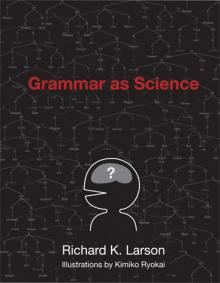
\includegraphics[height=5em]{./img/grammarasscience}
            \quad
            \phantom{a}
        \end{columns}
    \end{followup}
\end{frame}

\begin{frame}{Tree Bigrams}
    \begin{itemize}
        \item If sentences are tree structures, then a natural language is not a collection of strings but a collection of trees.
        \item But how can we describe these trees?
    \end{itemize}
    %
    \begin{block}{Tree Bigrams}
        A \textbf{tree bigram} consists of a node and one or more daughters:
        %
        \begin{center}
            \begin{forest}
                    [N, for tree={parent anchor=south, child anchor=north} 
                        [D$_1$]
                        [$\cdots$]
                        [$\cdots$]
                        [D$_n$]
                    ]
            \end{forest}
        \end{center}
    \end{block}
\end{frame}

\begin{frame}{Example: Tree Bigrams in \emph{cats bite dogs}}
    \begin{columns}
        \column{.4\linewidth}    
            \begin{forest}
                [S, for tree={parent anchor=south, child anchor=north}
                    [NP
                        [N [cats] ]
                    ]
                    [VP
                        [V [bite] ]
                        [NP
                            [N [dogs] ]
                        ]
                    ]
                ]
            \end{forest}

        \column{.6\linewidth}    
            \begin{tabular}{ccc}
                \begin{forest}
                    [S, for tree={parent anchor=south, child anchor=north}
                        [NP]
                        [VP]
                    ]
                \end{forest}
                &
                \begin{forest}
                    [NP, for tree={parent anchor=south, child anchor=north}
                        [N]
                    ]
                \end{forest}
                &
                \begin{forest}
                    [N, for tree={parent anchor=south, child anchor=north}
                        [cats]
                    ]
                \end{forest}
                \\
                \begin{forest}
                    [VP, for tree={parent anchor=south, child anchor=north}
                        [V]
                        [NP]
                    ]
                \end{forest}
                &
                \begin{forest}
                    [V, for tree={parent anchor=south, child anchor=north}
                        [bite]
                    ]
                \end{forest}
                &
                \begin{forest}
                    [N, for tree={parent anchor=south, child anchor=north}
                        [dogs]
                    ]
                \end{forest}
            \end{tabular}
    \end{columns}
\end{frame}

\begin{frame}{Tree Bigram Grammars}
    \begin{itemize}
        \item A \highlight{tree bigram grammar} is a collection of well-formed tree bigrams.
        \item Sentences are constructed by ``clicking'' tree bigrams together like Lego bricks.
    \end{itemize}

    \pause
    \begin{center}
        \begin{tabular}{cccccc}
            \begin{forest}
                [S, for tree={parent anchor=south, child anchor=north}
                    [NP]
                    [VP]
                ]
            \end{forest}
            &
            \begin{forest}
                [NP, for tree={parent anchor=south, child anchor=north}
                    [N]
                ]
            \end{forest}
            &
            \begin{forest}
                [NP, for tree={parent anchor=south, child anchor=north}
                    [Det]
                    [N]
                ]
            \end{forest}
            &
            \begin{forest}
                [VP, for tree={parent anchor=south, child anchor=north}
                    [V]
                ]
            \end{forest}
            &
            \begin{forest}
                [VP, for tree={parent anchor=south, child anchor=north}
                    [V]
                    [NP]
                ]
            \end{forest}
            &
            \begin{forest}
                [VP, for tree={parent anchor=south, child anchor=north}
                    [V]
                    [NP]
                    [NP]
                ]
            \end{forest}
        \end{tabular}

        \begin{tabular}{ccccccc}
            \begin{forest}
                [Det, for tree={parent anchor=south, child anchor=north}
                    [the]
                ]
            \end{forest}
            &
            \begin{forest}
                [Det, for tree={parent anchor=south, child anchor=north}
                    [a]
                ]
            \end{forest}
            &
            \begin{forest}
                [N, for tree={parent anchor=south, child anchor=north}
                    [cat]
                ]
            \end{forest}
            &
            \begin{forest}
                [N, for tree={parent anchor=south, child anchor=north}
                    [dogs]
                ]
            \end{forest}
            &
            \begin{forest}
                [V, for tree={parent anchor=south, child anchor=north}
                    [sleeps]
                ]
            \end{forest}
            &
            \begin{forest}
                [V, for tree={parent anchor=south, child anchor=north}
                    [bite]
                ]
            \end{forest}
            &
            \begin{forest}
                [V, for tree={parent anchor=south, child anchor=north}
                    [shows]
                ]
            \end{forest}
        \end{tabular}
    \end{center}
\end{frame}

\begin{frame}{Working with Tree Bigram Grammars: Verifying Trees}
    It is very easy to verify whether a given tree is licensed by a given grammar.

    \begin{block}{Algorithm: Determining Tree Well-Formedness}
        \textbf{Input:} grammar \colored{purple}{G} and tree \colored{teal}{$t$}\\
        \textbf{Output:} True if \colored{teal}{$t$} is well-formed, False otherwise
        \begin{enumerate}
            \item extract all tree bigrams of \colored{teal}{$t$}
            \item if at least one tree bigram is not in \colored{purple}{G}, return False
            \item otherwise, return True
        \end{enumerate}
    \end{block}
\end{frame}

\begin{frame}{Example: An Illicit Tree}
    \textbf{Tree Bigram Grammar:}\\
        \begin{center}
            \small
            \begin{tabular}{cccccc}
                \begin{forest}
                    [S, for tree={parent anchor=south, child anchor=north}
                        [NP]
                        [VP]
                    ]
                \end{forest}
                &
                \begin{forest}
                    [NP, for tree={parent anchor=south, child anchor=north}
                        [N]
                    ]
                \end{forest}
                &
                \begin{forest}
                    [N, for tree={parent anchor=south, child anchor=north}
                        [cats]
                    ]
                \end{forest}
                &
                \begin{forest}
                    [VP, for tree={parent anchor=south, child anchor=north}
                        [V]
                        [NP]
                    ]
                \end{forest}
                &
                \begin{forest}
                    [V, for tree={parent anchor=south, child anchor=north}
                        [bite]
                    ]
                \end{forest}
                &
                \begin{forest}
                    [N, for tree={parent anchor=south, child anchor=north}
                        [dogs]
                    ]
                \end{forest}
            \end{tabular}
        \end{center}

    \begin{columns}
        \column{.4\linewidth}
        \textbf{Input Tree:}\\
            \small
            \centering
            \begin{forest}
                [S, for tree={parent anchor=south, child anchor=north}
                    [NP,
                        [N,
                            [dogs]
                        ]
                    ]
                    [VP,
                        [V,
                            [bite]
                        ]
                        [NP,
                            [N,
                                [dogs]
                            ]
                        ]
                        [NP,
                            [N,
                                [dogs]
                            ]
                        ]
                    ]
                ]
            \end{forest}
        \column{.6\linewidth}
        \textbf{Extracted Tree Bigrams:}\\
            \small
            \quad
            \begin{tabular}{cccc}
                \begin{forest}
                    [S, for tree={parent anchor=south, child anchor=north}
                        [NP]
                        [VP]
                    ]
                \end{forest}
                &
                \begin{forest}
                    [NP, for tree={parent anchor=south, child anchor=north}
                        [N]
                    ]
                \end{forest}
                &
                \begin{forest}
                    [N, for tree={parent anchor=south, child anchor=north}
                        [dogs]
                    ]
                \end{forest}
                &
                \begin{forest}
                    [V, for tree={parent anchor=south, child anchor=north}
                        [bite]
                    ]
                \end{forest}
                \\
                \color{red}
                \begin{forest}
                    [VP, for tree={parent anchor=south, child anchor=north}
                        [V]
                        [NP]
                        [NP]
                    ]
                \end{forest}
            \end{tabular}
    \end{columns}
\end{frame}

\begin{frame}{Adding Probabilities}
    \begin{itemize}
        \item With bigrams it was often advantageous to add probabilities.\\
              This can also be done for tree bigrams.
        \item \textbf{Tree banks} are corpora where every sentence has been annotated with a tree structure.
        \item We can calculate the frequency of tree bigrams in tree banks\\
            and use those to determine various probabilities.
    \end{itemize}
    %
    \begin{block}{Two Types of Probability}
        \begin{description}
            \item[tree probability] product of probabilities of all tree bigram tokens
            \item[string probability] sum of tree probabilities of all trees for the string
        \end{description}
    \end{block}
\end{frame}

\begin{frame}{Example: Probabilities for an Ambiguous Sentence}
    \begin{center}
        \begin{tabular}{ccccccc}
            \tiny
            \begin{forest}
                [S, for tree={parent anchor=south, child anchor=north}
                    [NP]
                    [VP]
                ]
            \end{forest}
            &
            \tiny
            \begin{forest}
                [NP, for tree={parent anchor=south, child anchor=north}
                    [N]
                ]
            \end{forest}
            &
            \tiny
            \begin{forest}
                [NP, for tree={parent anchor=south, child anchor=north}
                    [Det]
                    [N]
                ]
            \end{forest}
            &
            \tiny
            \begin{forest}
                [NP, for tree={parent anchor=south, child anchor=north}
                    [NP]
                    [PP]
                ]
            \end{forest}
            &
            \tiny
            \begin{forest}
                [VP, for tree={parent anchor=south, child anchor=north}
                    [V]
                    [NP]
                ]
            \end{forest}
            &
            \tiny
            \begin{forest}
                [VP, for tree={parent anchor=south, child anchor=north}
                    [VP]
                    [PP]
                ]
            \end{forest}
            &
            \tiny
            \begin{forest}
                [PP, for tree={parent anchor=south, child anchor=north}
                    [P]
                    [NP]
                ]
            \end{forest}
            \\
            1 & .25 & .6 & .15 & .9 & .1 & 1
            \\
            \tiny
            \begin{forest}
                [N, for tree={parent anchor=south, child anchor=north}
                    [I]
                ]
            \end{forest}
            &
            \tiny
            \begin{forest}
                [N, for tree={parent anchor=south, child anchor=north}
                    [man]
                ]
            \end{forest}
            &
            \tiny
            \begin{forest}
                [N, for tree={parent anchor=south, child anchor=north}
                    [binoculars]
                ]
            \end{forest}
            &
            \tiny
            \begin{forest}
                [Det, for tree={parent anchor=south, child anchor=north}
                    [the]
                ]
            \end{forest}
            &
            \tiny
            \begin{forest}
                [V, for tree={parent anchor=south, child anchor=north}
                    [saw]
                ]
            \end{forest}
            &
            \tiny
            \begin{forest}
                [P, for tree={parent anchor=south, child anchor=north}
                    [with]
                ]
            \end{forest}
            \\
            .4 & .4 & .2 & 1 & 1 & 1
        \end{tabular}
    \end{center}

    \begin{center}
        \begin{tabular}{cc}
        \tiny
            \begin{forest}
                [S, name=l, for tree={parent anchor=south, child anchor=north}
                    [NP, name=l0
                        [N, name=l00
                            [I, name=l000]
                        ]
                    ]
                    [VP, name=l1
                        [V, name=l10
                            [saw, name=l100]
                        ]
                        [NP, name=l11
                            [NP, name=l110
                                [Det, name=l1100
                                    [the, name=l11000]
                                ]
                                [N, name=l1101
                                    [man, name=l11010]
                                ]
                            ]
                            [PP, name=l111
                                [P, name=l1110
                                    [with, name=l11100]
                                ]
                                [NP, name=l1111
                                    [N, name=l11110
                                        [binoculars, name=l111100]
                                    ]
                                ]
                            ]
                        ]
                    ]
                ]
            \end{forest}
            &
            \tiny
            \begin{forest}
                [S, for tree={parent anchor=south, child anchor=north}
                    [NP,
                        [N,
                            [I]
                        ]
                    ]
                    [VP,
                        [VP,
                            [V,
                                [saw]
                            ]
                            [NP,
                                [Det,
                                    [the]
                                ]
                                [N,
                                    [man]
                                ]
                            ]
                        ]
                        [PP,
                            [P,
                                [with]
                            ]
                            [NP,
                                [N,
                                    [binoculars]
                                ]
                            ]
                        ]
                    ]
                ]
            \end{forest}
            \\
        \end{tabular}

        \small
        \textbf{Left:} $1 \times .25 \times .4 \times .9 \times 1 \times .15 \times .6 \times 1 \times .4 \times 1 \times 1 \times .25 \times .2 = 0.016\%$\\
        \textbf{Right:}
        $1 \times .25 \times .4 \times .1 \times .9 \times 1 \times .6 \times 1 \times .4 \times 1 \times 1 \times .25 \times .2 = 0.011\%$
    \end{center}
\end{frame}


\begin{frame}{Building Trees}
    \begin{itemize}
        \item In practice, one hardly ever gets a full tree as input.
        \item Instead, one usually starts out with the strings of words and\\
            has to find the correct tree structure(s).
        \item The process of inferring tree structure is called \textbf{parsing},\\
            and it is \highlight{surprisingly difficult}.
    \end{itemize}

    \pause
    \begin{block}{Humans are Incredible Parsing Machines}
        \begin{itemize}
            \item Humans parse on-the-fly while listening\\
                $\Rightarrow$ real-time comprehension
            \item Even our best parsing algorithms take up to $\colored{orange}{n}^3$ steps,\\
                where $\colored{orange}{n}$ is the number of words in the sentence.
        \end{itemize}
        %
        \centering
        \begin{tabular}{l@{\hspace{2em}}rrrrrcr}
            \textbf{\# of words}     & 1 & 2 & 3 & 4 & 5 & $\cdots$ & 10\\
            \textbf{Computing steps} & 1 & 8 & 27 & 64 & 125 & $\cdots$ & 1000
        \end{tabular}
    \end{block}
\end{frame}

\begin{frame}{Why Parsing is Harder for Computers}
    \begin{itemize}
        \item Sentences can have multiple meanings, they are \textbf{ambiguous}.
        \item This is reflected in \highlight{different tree structures}.
    \end{itemize}
    %
    \begin{center}
        \footnotesize
        \begin{forest}
            [S, for tree={parent anchor=south, child anchor=north}
                [NP,
                    [N,
                        [I]
                    ]
                ]
                [VP,
                    [V,
                        [saw]
                    ]
                    [NP,
                        [NP,
                            [Det,
                                [the]
                            ]
                            [N,
                                [man]
                            ]
                        ]
                        [PP,
                            [P,
                                [with]
                            ]
                            [NP,
                                [N,
                                    [binoculars]
                                ]
                            ]
                        ]
                    ]
                ]
            ]
        \end{forest}
        %
        \begin{forest}
            [S, for tree={parent anchor=south, child anchor=north}
                [NP,
                    [N,
                        [I]
                    ]
                ]
                [VP,
                    [VP,
                        [V,
                            [saw]
                        ]
                        [NP,
                            [Det,
                                [the]
                            ]
                            [N,
                                [man]
                            ]
                        ]
                    ]
                    [PP,
                        [P,
                            [with]
                        ]
                        [NP,
                            [N,
                                [binoculars]
                            ]
                        ]
                    ]
                ]
            ]
        \end{forest}
    \end{center}
\end{frame}
    
\begin{frame}{Why Parsing is Harder for Computers [cont.]}
    \begin{itemize}
        \item But sentences are hardly ever ambiguous in context.
    \end{itemize}
    %
    \begin{center}
        \footnotesize
        \begin{forest}
            [S, for tree={parent anchor=south, child anchor=north}
                [NP,
                    [N,
                        [I]
                    ]
                ]
                [VP,
                    [V,
                        [ate]
                    ]
                    [NP,
                        [NP,
                            [Det,
                                [the]
                            ]
                            [N,
                                [meal]
                            ]
                        ]
                        [PP,
                            [P,
                                [with]
                            ]
                            [NP,
                                [N,
                                    [pork]
                                ]
                            ]
                        ]
                    ]
                ]
            ]
        \end{forest}
        %
        \begin{forest}
            [S, for tree={parent anchor=south, child anchor=north}
                [NP,
                    [N,
                        [I]
                    ]
                ]
                [VP,
                    [VP,
                        [V,
                            [ate]
                        ]
                        [NP,
                            [Det,
                                [the]
                            ]
                            [N,
                                [meal]
                            ]
                        ]
                    ]
                    [PP,
                        [P,
                            [with]
                        ]
                        [NP,
                            [N,
                                [chop sticks]
                            ]
                        ]
                    ]
                ]
            ]
        \end{forest}
    \end{center}
\end{frame}

\begin{frame}{Why Parsing is Harder for Computers [cont.]}
    \begin{itemize}
        \item Humans easily handle context and world knowledge.
        \item That's why humans do not entertain non-sensical\\ tree structures.
        \item Computers \highlight{build all these implausible trees}\\
            because they have no grasp of meaning. 
        \item It is this extra work that slows computers down.
    \end{itemize}
\end{frame}


\begin{frame}{Comparison to Parsing of Programming Languages}
    \begin{itemize}
        \item Programming languages also have hidden structure that is explicitly specified via a grammar written by the designer of the language.
        \item This hidden structure is required to translate the program into machine code.
        \item Programming languages are designed to be free of ambiguity.
        \item In this case, parsing is \textbf{deterministic} and runs at linear speed:\\ parsing a program with $n$ words takes $k \times n + d$ steps.
        % \item Linear is very fast, but it's still not quite as fast as humans.
    \end{itemize}

    \begin{block}{Moral of the Story}
        \begin{itemize}
            \item Without ambiguity, parsing is fast.
            \item Humans use meaning to keep ambiguity to a minimum.
        \end{itemize}
    \end{block}
\end{frame}

\begin{frame}{Trees Make Meaning Easier}
    \begin{block}{Central Idea}
        \begin{itemize}
            \item Tree structures encode important relations in sentence
            \item From the relations we can build the meaning.
        \end{itemize}
    \end{block}

    \textbf{Step 1}: Annotate tree with grammatical relations
    %
    \begin{center}
        \begin{forest}
            [S,name=s, s sep=5em
                [NP,name=subj
                    [Det,name=every
                        [every]
                    ]
                    [N,name=dog
                        [dog]
                    ]
                ]
                [VP,name=vp
                    [V,name=v
                        [chases]
                    ]
                    [NP,name=obj
                        [N,name=cat
                            [Mocha]
                        ]
                    ]
                ]
            ]
            %
            \foreach \Node/\Placement/\Role/\Counter in {%
                v/above left/predicate/2,
                obj/right/object/3,
                dog/right/domain/5,
                every/left/quantifier/5,
                subj/left/subject/4%
                }
                \node [\Placement=.05em of \Node,font={\footnotesize},align=center,SteelBlue4, visible on=<\Counter->] {\Role};
        \end{forest}
    \end{center}
\end{frame}

\begin{frame}{From Phrase Structure Tree to Dependencies}
    \textbf{Step 2:} Convert annotated tree to dependency tree
    %
    \begin{center}
        \begin{forest}
            [chases, name=chase
                [every, name=every
                    [dog, name=dog]
                ]
                [Moccha, name=mocha]
            ]
            \foreach \Node/\Placement/\Role/\Counter in {%
                mocha/above right/theme/2,
                every/above left/agent/3,
                dog/above left/domain/4%
                }
                \node [\Placement=.05em of \Node,font={\footnotesize},align=center,SteelBlue4, visible on=<\Counter->] {\Role};
        \end{forest}
    \end{center}
\end{frame}

\begin{frame}{From Dependencies to Meaning Representations}
    \textbf{Step 3:} Convert dependency tree to Abstract Meaning Representation (AMR)
    %
    \begin{center}
        \begin{tikzpicture}
            \node (every) at (0,0) {every};
            \node (dog) [below=2em of every] {dog};
            \node (middle) at ($(every)!.5!(dog)$) {\phantom{dog}};
            \node (Mocha) [right=8em of middle] {Mocha};

            \draw[dashed] (every.north west) rectangle (dog.south east);
            \draw[->] (middle) to node [above] {acts-on} node [below] {manner: chase} (Mocha);
        \end{tikzpicture}
    \end{center}

    \pause
    \begin{block}{What's the point?}
        \begin{itemize}
            \item AMRs encode the abstract meaning dependencies between sentence parts
            \item This allows us to build a full meaning:
                \begin{itemize}
                    \item Replace individual nodes by their lexical meaning (e.g.\ vectors)
                    \item Combine lexical meanings via operators that correspond to dependencies (e.g.\ dot product)
                \end{itemize}
        \end{itemize}
    \end{block}
\end{frame}
\end{document}
